\documentclass[uplatex,dvipdfmx,11pt]{jsarticle}
\usepackage{amsmath,amssymb,amsthm,mathtools}
\usepackage{geometry}
\usepackage{bm}
\usepackage{graphicx}
\usepackage{tikz}
\usetikzlibrary{arrows.meta,positioning}
\usepackage[unicode]{hyperref}
\providecommand{\cInv}{\cos^{-1}}
\providecommand{\E}{\mathrm{E}}
\providecommand{\V}{\mathrm{V}}
\providecommand{\Cov}{\mathrm{Cov}}
\geometry{margin=24mm}

\begin{document}
\begin{center}
{\LARGE\bfseries MORTRA 検証済み解答\par}
\vspace{1mm}
{\small 分野：整数・解析\qquad 問題・厳密解・図・証明経路・講評}
\end{center}
\vspace{1mm}
\hrule
\vspace{5mm}

\section*{問題}
$(1)\ e<1+\sqrt3$を示せ.\\
$(2) \displaystyle\int_{0}^{1}e^x \sin xdx$は整数か.

\section*{答え}
\(\begin{aligned}\text{(1)}\;&e<1 + \sqrt{3}\\\text{(2)}\;&\text{整数ではない。}\end{aligned}\)

\section*{解答}
\textbf{(1)}\quad \textbf{1.} 指数関数の級数から \[e=\sum_{k=0}^\infty\frac1{k!}=\sum_{k=0}^5\frac1{k!}+\sum_{k=6}^\infty\frac1{k!}\] と分ける。前半は \(\frac{163}{60}\) である。

\textbf{2.} \(k\ge6\) では \(k!\ge6!\,7^{k-6}\) であり、\(k\ge8\) では不等号は厳しい。従って \[\sum_{k=6}^\infty\frac1{k!}<\frac1{6!}\sum_{j=0}^\infty\frac1{7^j}=\frac{7}{4320}.\] よって \(e<\frac{11743}{4320}\) である。

\textbf{3.} さらに \(\frac{11743}{4320}<87/32\) である。一方、\[\left(\frac{87}{32}-1\right)^2=\frac{3025}{1024}<3\] であり、比較している数は正である。従って \(87/32<1+\sqrt{3}=1 + \sqrt{3}\) となる。

\textbf{4.} 以上より \[e<1 + \sqrt{3}\] が成り立つ。

\textbf{(2)}\quad \textbf{1.} \(0<x\le1\) とする。\(g(x)=x-\sin x\) とおけば \(g(0)=0\)、\(g'(x)=1-\cos x>0\) である。従って \(0<\sin x<x\) となる。

\textbf{2.} \(e^{x}>0\) を掛けて積分すると \[0<\int_0^1e^{x}\sin x\,dx<\int_0^1xe^{x}\,dx.\]

\textbf{3.} 右辺は部分積分により \[\int_0^1xe^{x}\,dx=\left[e^{x}(x-1)\right]_0^1=1.\]

\textbf{4.} 従って、求める積分値は0と1の間に厳密に入る。よって整数ではない。

\clearpage

\section*{一手ずつ見る図解}

\subsection*{1. e を正の級数へ移す}

第5項までを正確に足し、残りを独立した尾項として分けます。

\[
\sum_{k=0}^5\frac1{k!}=\frac{163}{60}
\]

\begin{center}

\begin{tikzpicture}[scale=2.192982,line cap=round,line join=round]
\path[use as bounding box] (-0.30000000,0.70000000) rectangle (5.40000000,3.00000000);
\draw[->,black!35] (0,0.70000000)--(0,3.00000000);
\draw[draw=cyan!65!black,line width=.7pt] (0.00000000,1.00000000) -- (1.00000000,2.00000000) -- (2.00000000,2.50000000) -- (3.00000000,2.66666667) -- (4.00000000,2.70833333) -- (5.00000000,2.71666667);
\fill[black!80] (0.00000000,1.00000000) circle (1.25pt);
\node[font=\scriptsize,anchor=south west,text=black!80] at (0.00000000,1.00000000) {S\_0};
\fill[black!80] (1.00000000,2.00000000) circle (1.25pt);
\node[font=\scriptsize,anchor=south west,text=black!80] at (1.00000000,2.00000000) {S\_1};
\fill[black!80] (2.00000000,2.50000000) circle (1.25pt);
\node[font=\scriptsize,anchor=south west,text=black!80] at (2.00000000,2.50000000) {S\_2};
\fill[black!80] (3.00000000,2.66666667) circle (1.25pt);
\node[font=\scriptsize,anchor=south west,text=black!80] at (3.00000000,2.66666667) {S\_3};
\fill[black!80] (4.00000000,2.70833333) circle (1.25pt);
\node[font=\scriptsize,anchor=south west,text=black!80] at (4.00000000,2.70833333) {S\_4};
\fill[magenta!70!black] (5.00000000,2.71666667) circle (1.25pt);
\node[font=\scriptsize,anchor=south west,text=magenta!70!black] at (5.00000000,2.71666667) {S\_5};
\end{tikzpicture}

\end{center}

\subsection*{2. 尾項を等比級数で抑える}

6次以降では分母が少なくとも毎回7倍になることを使います。

\[
e<\frac{163}{60}+\frac{7}{4320}=\frac{11743}{4320}<\frac{87}{32}
\]

\begin{center}


\begin{tikzpicture}[scale=7.500000,line cap=round,line join=round]
\path[use as bounding box] (2.63666667,-0.48000000) rectangle (2.79875000,0.48000000);
\draw[->,black!35] (2.63666667,0)--(2.79875000,0);
\draw[draw=black!38,line width=.7pt] (2.71666667,0.00000000) -- (2.71875000,0.00000000);
\draw[draw=cyan!65!black,line width=.7pt] (2.71666667,0.00000000) -- (2.71828704,0.00000000);
\fill[black!80] (2.71666667,0.00000000) circle (1.25pt);
\fill[magenta!70!black] (2.71666667,0.00000000) circle (1.25pt);
\fill[magenta!70!black] (2.71828704,0.00000000) circle (1.25pt);
\fill[black!80] (2.71875000,0.00000000) circle (1.25pt);
\node[font=\scriptsize,fill=white,inner sep=1.5pt] at (2.71666667,0.16000000) {\(S_5\)};
\node[font=\scriptsize,fill=white,inner sep=1.5pt] at (2.71666667,-0.16000000) {\(S_5\)};
\node[font=\scriptsize,fill=white,inner sep=1.5pt] at (2.71828704,0.16000000) {\(\frac{11743}{4320}\)};
\node[font=\scriptsize,fill=white,inner sep=1.5pt] at (2.71875000,-0.16000000) {\(\frac{87}{32}\)};
\end{tikzpicture}

\end{center}

\subsection*{3. 根号との大小を平方で決める}

両辺から1を引くと正なので、二乗した有理数の比較で結論が出ます。

\[
\left(\frac{87}{32}-1\right)^2=\frac{3025}{1024}<3
\]

\begin{center}

\begin{tikzpicture}[scale=5.306528,line cap=round,line join=round]
\path[use as bounding box] (0.68823085,-0.48000000) rectangle (3.04381995,0.48000000);
\draw[->,black!35] (0.68823085,0)--(3.04381995,0);
\draw[draw=black!38,line width=.7pt] (1.00000000,0.00000000) -- (2.73205081,0.00000000);
\draw[draw=cyan!65!black,line width=.7pt] (2.71828704,0.00000000) -- (2.71875000,0.00000000);
\fill[black!80] (1.00000000,0.00000000) circle (1.25pt);
\fill[magenta!70!black] (2.71828704,0.00000000) circle (1.25pt);
\fill[magenta!70!black] (2.71875000,0.00000000) circle (1.25pt);
\fill[black!80] (2.73205081,0.00000000) circle (1.25pt);
\node[font=\scriptsize,fill=white,inner sep=1.5pt] at (1.00000000,0.16000000) {\(1\)};
\node[font=\scriptsize,fill=white,inner sep=1.5pt] at (2.71828704,-0.16000000) {\(e_{\mathrm{upper}}\)};
\node[font=\scriptsize,fill=white,inner sep=1.5pt] at (2.71875000,0.16000000) {\(\frac{87}{32}\)};
\node[font=\scriptsize,fill=white,inner sep=1.5pt] at (2.73205081,-0.16000000) {\(1 + \sqrt{3}\)};
\end{tikzpicture}

\end{center}

\subsection*{4. 正弦を直線と比較する}

正弦と直線の差を微分し、区間の内部で正弦が直線より下にあることを確定します。

\[
0<\sin x<x\qquad(0<x\le1)
\]

\begin{center}

\begin{tikzpicture}[scale=3.752438,line cap=round,line join=round]
\path[use as bounding box] (0.00000000,-0.47500260) rectangle (1.00000000,1.44375000);
\draw[->,black!35] (0.00000000,0)--(1.00000000,0);
\draw[->,black!35] (0,-0.47500260)--(0,1.44375000);
\draw[draw=cyan!65!black,line width=.7pt] (0.00000000,0.00000000) -- (0.00625000,0.00624996) -- (0.01250000,0.01249967) -- (0.01875000,0.01874890) -- (0.02500000,0.02499740) -- (0.03125000,0.03124491) -- (0.03750000,0.03749121) -- (0.04375000,0.04373604) -- (0.05000000,0.04997917) -- (0.05625000,0.05622034) -- (0.06250000,0.06245932) -- (0.06875000,0.06869585) -- (0.07500000,0.07492971) -- (0.08125000,0.08116063) -- (0.08750000,0.08738839) -- (0.09375000,0.09361273) -- (0.10000000,0.09983342) -- (0.10625000,0.10605020) -- (0.11250000,0.11226285) -- (0.11875000,0.11847110) -- (0.12500000,0.12467473) -- (0.13125000,0.13087349) -- (0.13750000,0.13706714) -- (0.14375000,0.14325543) -- (0.15000000,0.14943813) -- (0.15625000,0.15561499) -- (0.16250000,0.16178577) -- (0.16875000,0.16795024) -- (0.17500000,0.17410814) -- (0.18125000,0.18025924) -- (0.18750000,0.18640330) -- (0.19375000,0.19254007) -- (0.20000000,0.19866933) -- (0.20625000,0.20479083) -- (0.21250000,0.21090432) -- (0.21875000,0.21700958) -- (0.22500000,0.22310636) -- (0.23125000,0.22919443) -- (0.23750000,0.23527354) -- (0.24375000,0.24134346) -- (0.25000000,0.24740396) -- (0.25625000,0.25345479) -- (0.26250000,0.25949572) -- (0.26875000,0.26552652) -- (0.27500000,0.27154694) -- (0.28125000,0.27755675) -- (0.28750000,0.28355572) -- (0.29375000,0.28954362) -- (0.30000000,0.29552021) -- (0.30625000,0.30148525) -- (0.31250000,0.30743851) -- (0.31875000,0.31337977) -- (0.32500000,0.31930879) -- (0.33125000,0.32522533) -- (0.33750000,0.33112917) -- (0.34375000,0.33702007) -- (0.35000000,0.34289781) -- (0.35625000,0.34876215) -- (0.36250000,0.35461287) -- (0.36875000,0.36044974) -- (0.37500000,0.36627253) -- (0.38125000,0.37208101) -- (0.38750000,0.37787496) -- (0.39375000,0.38365414) -- (0.40000000,0.38941834) -- (0.40625000,0.39516733) -- (0.41250000,0.40090088) -- (0.41875000,0.40661877) -- (0.42500000,0.41232078) -- (0.43125000,0.41800668) -- (0.43750000,0.42367626) -- (0.44375000,0.42932928) -- (0.45000000,0.43496553) -- (0.45625000,0.44058480) -- (0.46250000,0.44618685) -- (0.46875000,0.45177147) -- (0.47500000,0.45733845) -- (0.48125000,0.46288756) -- (0.48750000,0.46841859) -- (0.49375000,0.47393132) -- (0.50000000,0.47942554) -- (0.50625000,0.48490103) -- (0.51250000,0.49035758) -- (0.51875000,0.49579498) -- (0.52500000,0.50121300) -- (0.53125000,0.50661145) -- (0.53750000,0.51199012) -- (0.54375000,0.51734878) -- (0.55000000,0.52268723) -- (0.55625000,0.52800526) -- (0.56250000,0.53330267) -- (0.56875000,0.53857925) -- (0.57500000,0.54383479) -- (0.58125000,0.54906909) -- (0.58750000,0.55428193) -- (0.59375000,0.55947313) -- (0.60000000,0.56464247) -- (0.60625000,0.56978976) -- (0.61250000,0.57491479) -- (0.61875000,0.58001736) -- (0.62500000,0.58509727) -- (0.63125000,0.59015433) -- (0.63750000,0.59518834) -- (0.64375000,0.60019909) -- (0.65000000,0.60518641) -- (0.65625000,0.61015008) -- (0.66250000,0.61508991) -- (0.66875000,0.62000573) -- (0.67500000,0.62489732) -- (0.68125000,0.62976450) -- (0.68750000,0.63460708) -- (0.69375000,0.63942487) -- (0.70000000,0.64421769) -- (0.70625000,0.64898534) -- (0.71250000,0.65372764) -- (0.71875000,0.65844440) -- (0.72500000,0.66313544) -- (0.73125000,0.66780058) -- (0.73750000,0.67243964) -- (0.74375000,0.67705242) -- (0.75000000,0.68163876) -- (0.75625000,0.68619847) -- (0.76250000,0.69073138) -- (0.76875000,0.69523731) -- (0.77500000,0.69971608) -- (0.78125000,0.70416751) -- (0.78750000,0.70859144) -- (0.79375000,0.71298769) -- (0.80000000,0.71735609) -- (0.80625000,0.72169647) -- (0.81250000,0.72600866) -- (0.81875000,0.73029248) -- (0.82500000,0.73454778) -- (0.83125000,0.73877439) -- (0.83750000,0.74297214) -- (0.84375000,0.74714086) -- (0.85000000,0.75128041) -- (0.85625000,0.75539060) -- (0.86250000,0.75947129) -- (0.86875000,0.76352231) -- (0.87500000,0.76754350) -- (0.88125000,0.77153472) -- (0.88750000,0.77549579) -- (0.89375000,0.77942657) -- (0.90000000,0.78332691) -- (0.90625000,0.78719665) -- (0.91250000,0.79103564) -- (0.91875000,0.79484372) -- (0.92500000,0.79862076) -- (0.93125000,0.80236661) -- (0.93750000,0.80608111) -- (0.94375000,0.80976412) -- (0.95000000,0.81341550) -- (0.95625000,0.81703511) -- (0.96250000,0.82062281) -- (0.96875000,0.82417844) -- (0.97500000,0.82770189) -- (0.98125000,0.83119300) -- (0.98750000,0.83465164) -- (0.99375000,0.83807768) -- (1.00000000,0.84147098);
\draw[draw=black!80,line width=.7pt] (0.00000000,0.00000000) -- (0.00625000,0.00625000) -- (0.01250000,0.01250000) -- (0.01875000,0.01875000) -- (0.02500000,0.02500000) -- (0.03125000,0.03125000) -- (0.03750000,0.03750000) -- (0.04375000,0.04375000) -- (0.05000000,0.05000000) -- (0.05625000,0.05625000) -- (0.06250000,0.06250000) -- (0.06875000,0.06875000) -- (0.07500000,0.07500000) -- (0.08125000,0.08125000) -- (0.08750000,0.08750000) -- (0.09375000,0.09375000) -- (0.10000000,0.10000000) -- (0.10625000,0.10625000) -- (0.11250000,0.11250000) -- (0.11875000,0.11875000) -- (0.12500000,0.12500000) -- (0.13125000,0.13125000) -- (0.13750000,0.13750000) -- (0.14375000,0.14375000) -- (0.15000000,0.15000000) -- (0.15625000,0.15625000) -- (0.16250000,0.16250000) -- (0.16875000,0.16875000) -- (0.17500000,0.17500000) -- (0.18125000,0.18125000) -- (0.18750000,0.18750000) -- (0.19375000,0.19375000) -- (0.20000000,0.20000000) -- (0.20625000,0.20625000) -- (0.21250000,0.21250000) -- (0.21875000,0.21875000) -- (0.22500000,0.22500000) -- (0.23125000,0.23125000) -- (0.23750000,0.23750000) -- (0.24375000,0.24375000) -- (0.25000000,0.25000000) -- (0.25625000,0.25625000) -- (0.26250000,0.26250000) -- (0.26875000,0.26875000) -- (0.27500000,0.27500000) -- (0.28125000,0.28125000) -- (0.28750000,0.28750000) -- (0.29375000,0.29375000) -- (0.30000000,0.30000000) -- (0.30625000,0.30625000) -- (0.31250000,0.31250000) -- (0.31875000,0.31875000) -- (0.32500000,0.32500000) -- (0.33125000,0.33125000) -- (0.33750000,0.33750000) -- (0.34375000,0.34375000) -- (0.35000000,0.35000000) -- (0.35625000,0.35625000) -- (0.36250000,0.36250000) -- (0.36875000,0.36875000) -- (0.37500000,0.37500000) -- (0.38125000,0.38125000) -- (0.38750000,0.38750000) -- (0.39375000,0.39375000) -- (0.40000000,0.40000000) -- (0.40625000,0.40625000) -- (0.41250000,0.41250000) -- (0.41875000,0.41875000) -- (0.42500000,0.42500000) -- (0.43125000,0.43125000) -- (0.43750000,0.43750000) -- (0.44375000,0.44375000) -- (0.45000000,0.45000000) -- (0.45625000,0.45625000) -- (0.46250000,0.46250000) -- (0.46875000,0.46875000) -- (0.47500000,0.47500000) -- (0.48125000,0.48125000) -- (0.48750000,0.48750000) -- (0.49375000,0.49375000) -- (0.50000000,0.50000000) -- (0.50625000,0.50625000) -- (0.51250000,0.51250000) -- (0.51875000,0.51875000) -- (0.52500000,0.52500000) -- (0.53125000,0.53125000) -- (0.53750000,0.53750000) -- (0.54375000,0.54375000) -- (0.55000000,0.55000000) -- (0.55625000,0.55625000) -- (0.56250000,0.56250000) -- (0.56875000,0.56875000) -- (0.57500000,0.57500000) -- (0.58125000,0.58125000) -- (0.58750000,0.58750000) -- (0.59375000,0.59375000) -- (0.60000000,0.60000000) -- (0.60625000,0.60625000) -- (0.61250000,0.61250000) -- (0.61875000,0.61875000) -- (0.62500000,0.62500000) -- (0.63125000,0.63125000) -- (0.63750000,0.63750000) -- (0.64375000,0.64375000) -- (0.65000000,0.65000000) -- (0.65625000,0.65625000) -- (0.66250000,0.66250000) -- (0.66875000,0.66875000) -- (0.67500000,0.67500000) -- (0.68125000,0.68125000) -- (0.68750000,0.68750000) -- (0.69375000,0.69375000) -- (0.70000000,0.70000000) -- (0.70625000,0.70625000) -- (0.71250000,0.71250000) -- (0.71875000,0.71875000) -- (0.72500000,0.72500000) -- (0.73125000,0.73125000) -- (0.73750000,0.73750000) -- (0.74375000,0.74375000) -- (0.75000000,0.75000000) -- (0.75625000,0.75625000) -- (0.76250000,0.76250000) -- (0.76875000,0.76875000) -- (0.77500000,0.77500000) -- (0.78125000,0.78125000) -- (0.78750000,0.78750000) -- (0.79375000,0.79375000) -- (0.80000000,0.80000000) -- (0.80625000,0.80625000) -- (0.81250000,0.81250000) -- (0.81875000,0.81875000) -- (0.82500000,0.82500000) -- (0.83125000,0.83125000) -- (0.83750000,0.83750000) -- (0.84375000,0.84375000) -- (0.85000000,0.85000000) -- (0.85625000,0.85625000) -- (0.86250000,0.86250000) -- (0.86875000,0.86875000) -- (0.87500000,0.87500000) -- (0.88125000,0.88125000) -- (0.88750000,0.88750000) -- (0.89375000,0.89375000) -- (0.90000000,0.90000000) -- (0.90625000,0.90625000) -- (0.91250000,0.91250000) -- (0.91875000,0.91875000) -- (0.92500000,0.92500000) -- (0.93125000,0.93125000) -- (0.93750000,0.93750000) -- (0.94375000,0.94375000) -- (0.95000000,0.95000000) -- (0.95625000,0.95625000) -- (0.96250000,0.96250000) -- (0.96875000,0.96875000) -- (0.97500000,0.97500000) -- (0.98125000,0.98125000) -- (0.98750000,0.98750000) -- (0.99375000,0.99375000) -- (1.00000000,1.00000000);
\end{tikzpicture}

\end{center}

\subsection*{5. 正の指数関数を掛けて積分する}

正の関数を掛けた後も不等号は保たれ、区間全体の積分へ移せます。

\[
0<e^{x}\sin x<xe^{x}
\]

\begin{center}

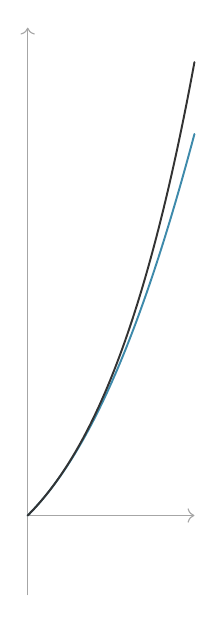
\begin{tikzpicture}[scale=2.118003,line cap=round,line join=round]
\path[use as bounding box] (0.00000000,-0.47436979) rectangle (1.00000000,2.92505941);
\draw[->,black!35] (0.00000000,0)--(1.00000000,0);
\draw[->,black!35] (0,-0.47436979)--(0,2.92505941);
\draw[draw=cyan!65!black,line width=.7pt] (0.00000000,0.00000000) -- (0.00625000,0.00628914) -- (0.01250000,0.01265690) -- (0.01875000,0.01910376) -- (0.02500000,0.02563021) -- (0.03125000,0.03223673) -- (0.03750000,0.03892383) -- (0.04375000,0.04569197) -- (0.05000000,0.05254166) -- (0.05625000,0.05947337) -- (0.06250000,0.06648760) -- (0.06875000,0.07358483) -- (0.07500000,0.08076554) -- (0.08125000,0.08803023) -- (0.08750000,0.09537938) -- (0.09375000,0.10281347) -- (0.10000000,0.11033299) -- (0.10625000,0.11793842) -- (0.11250000,0.12563024) -- (0.11875000,0.13340893) -- (0.12500000,0.14127498) -- (0.13125000,0.14922887) -- (0.13750000,0.15727107) -- (0.14375000,0.16540207) -- (0.15000000,0.17362234) -- (0.15625000,0.18193236) -- (0.16250000,0.19033260) -- (0.16875000,0.19882354) -- (0.17500000,0.20740566) -- (0.18125000,0.21607942) -- (0.18750000,0.22484530) -- (0.19375000,0.23370376) -- (0.20000000,0.24265527) -- (0.20625000,0.25170030) -- (0.21250000,0.26083932) -- (0.21875000,0.27007279) -- (0.22500000,0.27940117) -- (0.23125000,0.28882492) -- (0.23750000,0.29834449) -- (0.24375000,0.30796036) -- (0.25000000,0.31767297) -- (0.25625000,0.32748278) -- (0.26250000,0.33739023) -- (0.26875000,0.34739578) -- (0.27500000,0.35749987) -- (0.28125000,0.36770295) -- (0.28750000,0.37800547) -- (0.29375000,0.38840786) -- (0.30000000,0.39891055) -- (0.30625000,0.40951400) -- (0.31250000,0.42021863) -- (0.31875000,0.43102487) -- (0.32500000,0.44193315) -- (0.33125000,0.45294389) -- (0.33750000,0.46405753) -- (0.34375000,0.47527448) -- (0.35000000,0.48659515) -- (0.35625000,0.49801997) -- (0.36250000,0.50954934) -- (0.36875000,0.52118368) -- (0.37500000,0.53292339) -- (0.38125000,0.54476886) -- (0.38750000,0.55672051) -- (0.39375000,0.56877873) -- (0.40000000,0.58094390) -- (0.40625000,0.59321642) -- (0.41250000,0.60559668) -- (0.41875000,0.61808505) -- (0.42500000,0.63068192) -- (0.43125000,0.64338765) -- (0.43750000,0.65620262) -- (0.44375000,0.66912720) -- (0.45000000,0.68216175) -- (0.45625000,0.69530662) -- (0.46250000,0.70856217) -- (0.46875000,0.72192876) -- (0.47500000,0.73540672) -- (0.48125000,0.74899639) -- (0.48750000,0.76269813) -- (0.49375000,0.77651225) -- (0.50000000,0.79043908) -- (0.50625000,0.80447896) -- (0.51250000,0.81863219) -- (0.51875000,0.83289908) -- (0.52500000,0.84727996) -- (0.53125000,0.86177511) -- (0.53750000,0.87638485) -- (0.54375000,0.89110945) -- (0.55000000,0.90594922) -- (0.55625000,0.92090442) -- (0.56250000,0.93597534) -- (0.56875000,0.95116225) -- (0.57500000,0.96646541) -- (0.58125000,0.98188508) -- (0.58750000,0.99742152) -- (0.59375000,1.01307496) -- (0.60000000,1.02884567) -- (0.60625000,1.04473386) -- (0.61250000,1.06073976) -- (0.61875000,1.07686361) -- (0.62500000,1.09310561) -- (0.63125000,1.10946598) -- (0.63750000,1.12594492) -- (0.64375000,1.14254262) -- (0.65000000,1.15925927) -- (0.65625000,1.17609506) -- (0.66250000,1.19305015) -- (0.66875000,1.21012473) -- (0.67500000,1.22731894) -- (0.68125000,1.24463294) -- (0.68750000,1.26206688) -- (0.69375000,1.27962089) -- (0.70000000,1.29729511) -- (0.70625000,1.31508966) -- (0.71250000,1.33300465) -- (0.71875000,1.35104019) -- (0.72500000,1.36919637) -- (0.73125000,1.38747330) -- (0.73750000,1.40587104) -- (0.74375000,1.42438967) -- (0.75000000,1.44302927) -- (0.75625000,1.46178987) -- (0.76250000,1.48067154) -- (0.76875000,1.49967431) -- (0.77500000,1.51879820) -- (0.78125000,1.53804325) -- (0.78750000,1.55740945) -- (0.79375000,1.57689682) -- (0.80000000,1.59650534) -- (0.80625000,1.61623500) -- (0.81250000,1.63608576) -- (0.81875000,1.65605760) -- (0.82500000,1.67615046) -- (0.83125000,1.69636428) -- (0.83750000,1.71669901) -- (0.84375000,1.73715455) -- (0.85000000,1.75773083) -- (0.85625000,1.77842775) -- (0.86250000,1.79924519) -- (0.86875000,1.82018303) -- (0.87500000,1.84124114) -- (0.88125000,1.86241939) -- (0.88750000,1.88371761) -- (0.89375000,1.90513564) -- (0.90000000,1.92667330) -- (0.90625000,1.94833041) -- (0.91250000,1.97010677) -- (0.91875000,1.99200216) -- (0.92500000,2.01401635) -- (0.93125000,2.03614913) -- (0.93750000,2.05840022) -- (0.94375000,2.08076938) -- (0.95000000,2.10325633) -- (0.95625000,2.12586078) -- (0.96250000,2.14858244) -- (0.96875000,2.17142099) -- (0.97500000,2.19437611) -- (0.98125000,2.21744745) -- (0.98750000,2.24063468) -- (0.99375000,2.26393742) -- (1.00000000,2.28735529);
\draw[draw=black!80,line width=.7pt] (0.00000000,0.00000000) -- (0.00625000,0.00628918) -- (0.01250000,0.01265723) -- (0.01875000,0.01910488) -- (0.02500000,0.02563288) -- (0.03125000,0.03224198) -- (0.03750000,0.03893295) -- (0.04375000,0.04570655) -- (0.05000000,0.05256355) -- (0.05625000,0.05950474) -- (0.06250000,0.06653090) -- (0.06875000,0.07364283) -- (0.07500000,0.08084131) -- (0.08125000,0.08812716) -- (0.08750000,0.09550120) -- (0.09375000,0.10296423) -- (0.10000000,0.11051709) -- (0.10625000,0.11816061) -- (0.11250000,0.12589563) -- (0.11875000,0.13372299) -- (0.12500000,0.14164356) -- (0.13125000,0.14965818) -- (0.13750000,0.15776773) -- (0.14375000,0.16597309) -- (0.15000000,0.17427514) -- (0.15625000,0.18267476) -- (0.16250000,0.19117285) -- (0.16875000,0.19977032) -- (0.17500000,0.20846809) -- (0.18125000,0.21726706) -- (0.18750000,0.22616817) -- (0.19375000,0.23517235) -- (0.20000000,0.24428055) -- (0.20625000,0.25349371) -- (0.21250000,0.26281280) -- (0.21875000,0.27223877) -- (0.22500000,0.28177261) -- (0.23125000,0.29141529) -- (0.23750000,0.30116781) -- (0.24375000,0.31103116) -- (0.25000000,0.32100635) -- (0.25625000,0.33109440) -- (0.26250000,0.34129632) -- (0.26875000,0.35161315) -- (0.27500000,0.36204594) -- (0.28125000,0.37259571) -- (0.28750000,0.38326355) -- (0.29375000,0.39405050) -- (0.30000000,0.40495764) -- (0.30625000,0.41598606) -- (0.31250000,0.42713686) -- (0.31875000,0.43841112) -- (0.32500000,0.44980996) -- (0.33125000,0.46133450) -- (0.33750000,0.47298587) -- (0.34375000,0.48476520) -- (0.35000000,0.49667364) -- (0.35625000,0.50871235) -- (0.36250000,0.52088249) -- (0.36875000,0.53318524) -- (0.37500000,0.54562178) -- (0.38125000,0.55819331) -- (0.38750000,0.57090102) -- (0.39375000,0.58374614) -- (0.40000000,0.59672988) -- (0.40625000,0.60985348) -- (0.41250000,0.62311819) -- (0.41875000,0.63652525) -- (0.42500000,0.65007593) -- (0.43125000,0.66377150) -- (0.43750000,0.67761326) -- (0.44375000,0.69160248) -- (0.45000000,0.70574048) -- (0.45625000,0.72002858) -- (0.46250000,0.73446809) -- (0.46875000,0.74906037) -- (0.47500000,0.76380674) -- (0.48125000,0.77870858) -- (0.48750000,0.79376726) -- (0.49375000,0.80898414) -- (0.50000000,0.82436064) -- (0.50625000,0.83989814) -- (0.51250000,0.85559806) -- (0.51875000,0.87146183) -- (0.52500000,0.88749090) -- (0.53125000,0.90368669) -- (0.53750000,0.92005068) -- (0.54375000,0.93658435) -- (0.55000000,0.95328916) -- (0.55625000,0.97016662) -- (0.56250000,0.98721824) -- (0.56875000,1.00444554) -- (0.57500000,1.02185005) -- (0.58125000,1.03943332) -- (0.58750000,1.05719690) -- (0.59375000,1.07514236) -- (0.60000000,1.09327128) -- (0.60625000,1.11158527) -- (0.61250000,1.13008592) -- (0.61875000,1.14877486) -- (0.62500000,1.16765372) -- (0.63125000,1.18672416) -- (0.63750000,1.20598782) -- (0.64375000,1.22544638) -- (0.65000000,1.24510154) -- (0.65625000,1.26495498) -- (0.66250000,1.28500843) -- (0.66875000,1.30526361) -- (0.67500000,1.32572226) -- (0.68125000,1.34638614) -- (0.68750000,1.36725701) -- (0.69375000,1.38833666) -- (0.70000000,1.40962690) -- (0.70625000,1.43112952) -- (0.71250000,1.45284635) -- (0.71875000,1.47477924) -- (0.72500000,1.49693005) -- (0.73125000,1.51930063) -- (0.73750000,1.54189289) -- (0.74375000,1.56470871) -- (0.75000000,1.58775001) -- (0.75625000,1.61101873) -- (0.76250000,1.63451681) -- (0.76875000,1.65824620) -- (0.77500000,1.68220890) -- (0.78125000,1.70640688) -- (0.78750000,1.73084217) -- (0.79375000,1.75551677) -- (0.80000000,1.78043274) -- (0.80625000,1.80559213) -- (0.81250000,1.83099701) -- (0.81875000,1.85664948) -- (0.82500000,1.88255163) -- (0.83125000,1.90870559) -- (0.83750000,1.93511351) -- (0.84375000,1.96177753) -- (0.85000000,1.98869982) -- (0.85625000,2.01588259) -- (0.86250000,2.04332804) -- (0.86875000,2.07103839) -- (0.87500000,2.09901588) -- (0.88125000,2.12726278) -- (0.88750000,2.15578137) -- (0.89375000,2.18457394) -- (0.90000000,2.21364280) -- (0.90625000,2.24299029) -- (0.91250000,2.27261876) -- (0.91875000,2.30253058) -- (0.92500000,2.33272814) -- (0.93125000,2.36321384) -- (0.93750000,2.39399012) -- (0.94375000,2.42505941) -- (0.95000000,2.45642418) -- (0.95625000,2.48808691) -- (0.96250000,2.52005011) -- (0.96875000,2.55231630) -- (0.97500000,2.58488803) -- (0.98125000,2.61776785) -- (0.98750000,2.65095835) -- (0.99375000,2.68446214) -- (1.00000000,2.71828183);
\end{tikzpicture}

\end{center}

\subsection*{6. 連続する二整数の間に置く}

上側の積分は部分積分でちょうど1になります。元の積分は0より大きく1より小さいため整数ではありません。

\[
0<\int_0^1e^{x}\sin x\,dx<\int_0^1xe^{x}\,dx=1
\]

\begin{center}

\begin{tikzpicture}[scale=7.500000,line cap=round,line join=round]
\path[use as bounding box] (-0.14000000,-0.48000000) rectangle (1.14000000,0.48000000);
\draw[->,black!35] (-0.14000000,0)--(1.14000000,0);
\draw[->,black!35] (0,-0.48000000)--(0,0.48000000);
\draw[draw=cyan!65!black,line width=.7pt] (0.00000000,0.00000000) -- (1.00000000,0.00000000);
\fill[black!80] (0.00000000,0.00000000) circle (1.25pt);
\node[font=\scriptsize,anchor=south west,text=black!80] at (0.00000000,0.00000000) {0};
\fill[black!80] (1.00000000,0.00000000) circle (1.25pt);
\node[font=\scriptsize,anchor=south west,text=black!80] at (1.00000000,0.00000000) {1};
\node[font=\scriptsize,fill=white,inner sep=1.5pt] at (0.50000000,0.20000000) {\(0<I<1\)};
\end{tikzpicture}

\end{center}

\section*{講評}
\noindent\textbf{出題意図}\quad 整数・解析の条件を実行可能な関係へ移し、設問ごとに分ける、共通条件を各設問へ引き継ぐ、各設問の証明書を再生するを一つの証明として組み立てる力を問う。

\noindent\textbf{想定する入試}\quad 記述式の大学入試または数学コンテストを想定し、変換の根拠と最終検証までを採点対象とする。

\noindent\textbf{独自性}\quad 数値近似や答えの照合で終えず、問題文から答えまで実際に通過した射と証明義務を再生できる。


\section*{証明の経路}
\begin{center}
\begin{tikzpicture}[
  node distance=3.5mm,
  stage/.style={draw,rounded corners=1pt,align=left,text width=118mm,minimum height=7mm,inner xsep=4pt,inner ysep=2pt,font=\small},
  flow/.style={-{Latex[length=2mm]},thick,cyan!55!black},
  edge label/.style={fill=white,inner xsep=3pt,font=\scriptsize\bfseries}
]
\node[stage] (n0) {問題文};
\node[stage,below=of n0] (n1) {番号付きの設問};
\draw[flow] (n0) -- node[edge label] {設問ごとに分ける} (n1);
\node[stage,below=of n1] (n2) {共通条件を引き継いだ各設問};
\draw[flow] (n1) -- node[edge label] {共通条件を各設問へ引き継ぐ} (n2);
\node[stage,below=of n2] (n3) {再生済みの部分証明};
\draw[flow] (n2) -- node[edge label] {各設問の証明書を再生する} (n3);
\node[stage,below=of n3] (n4) {全設問の検証済み解答};
\draw[flow] (n3) -- node[edge label] {全設問の証明を一つにまとめる} (n4);
\end{tikzpicture}
\end{center}

\clearpage
\section*{使った射と役割}
\begin{itemize}
\item \textbf{M1: 設問ごとに分ける}\\
問題文
$\longrightarrow$
番号付きの設問\\
共通の問題文を保ったまま、求める内容を番号付きの設問へ分ける。
\item \textbf{M2: 共通条件を各設問へ引き継ぐ}\\
番号付きの設問
$\longrightarrow$
共通条件を引き継いだ各設問\\
数列の定義と初期値を各設問へ引き継ぎ、四つの証明対象を確定する。
\item \textbf{M3: 各設問の証明書を再生する}\\
共通条件を引き継いだ各設問
$\longrightarrow$
再生済みの部分証明\\
各設問の計算と論証を独立に再実行し、全ての結論を検証する。
\item \textbf{M4: 全設問の証明を一つにまとめる}\\
再生済みの部分証明
$\longrightarrow$
全設問の検証済み解答\\
独立に検証した四つの結論を、元の問題に対する一つの解答としてまとめる。
\end{itemize}


\section*{証明義務}
\begin{itemize}
\item \textbf{設問(1)}: 証明義務 （検証済み）
\item \textbf{設問(2)}: 証明義務 （検証済み）
\end{itemize}


\section*{検証記録}
\begin{itemize}
\item 問題文を2個の設問へ構文分解
\item 共有条件を各設問の型付き意味表現へ継承
\item 各設問を独立に厳密実行
\item 全設問の証明書を再生し、全てが成立することを確認
\item 問題文・解答・検証証明書を出力
\end{itemize}
\noindent\textbf{検証方法}\quad 各設問の証明書を独立に再生し、全ての成立を確認
\par\noindent{\footnotesize 証明書 SHA-256: \nolinkurl{6cacedccaa6319bd426b0673d05b84dbba2e2b3c01eb0a4270de27a7c6d5aea4}}

\end{document}
